\colorlet{shadecolor}{\chapterColor}
\chapter{Quartzville Creek}\label{a:Quartzville Creek}
\markboth{\color{white}Quartzville Creek \protect\thepage \hspace{4pt}}{}
\lhead{\textcolor{\chapterColor}{\rule[-2pt]{\textwidth}{15pt}}}
About an hour further down the road from the main area there are a few interesting boulders in a creek. Generally lower temperatures, free camping, and pleasant swimming holes make this a nice mid summer spot.
\begin{figure}[h]
  \centering
    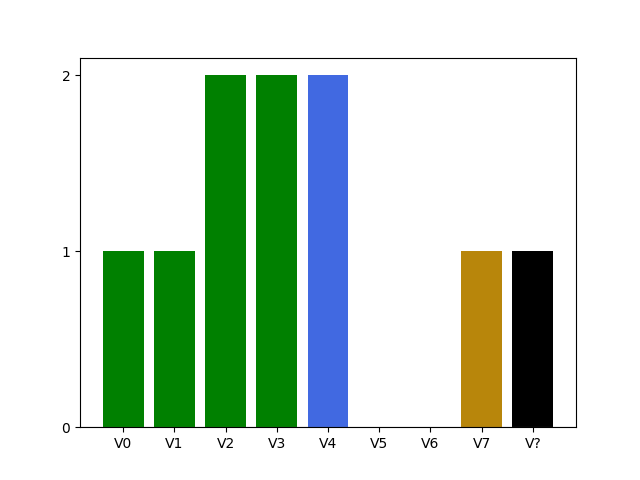
\includegraphics[width=\linewidth]{./maps/plots/Quartzville Creek.png}
\end{figure}

\section{Redneck Riviera}\label{sa:Redneck Riviera}
\qrcode{./maps/qr/Redneck Riviera_qr.png}{http://maps.google.com/maps?q=44.570410945356336,-122.4060701729652}{Navigate to this sub area}
Redneck rivierra is located on Quartzville road apporximately 20.6 miles from highway 20 park in the gravel pull out on the creek side of the road. This is a nice spot with good swimming access and a few established routes on both sides of the river. The locals like to use this spot to pan for gold. In my experience they are friendly and willing to share the space.
\subsection*{Pony Boy}\label{bf:Pony Boy}
\

\begin{enumerate}[]
	\setcounter{enumi}{0}
	\item\label{rt:Pony Boy} \colorbox{green!20}{\textbf{Pony Boy V2 \ding{73} } }
	\newline (No Topo) 
	\newline PLACEHOLDER\
\end{enumerate}
\subsection*{Monorail}\label{bf:Monorail}
\

\begin{enumerate}[]
	\setcounter{enumi}{1}
	\item\label{rt:Monorail Project} \colorbox{black!20}{\textbf{Monorail Project V?  } }
	\newline (No Topo) 
	\newline Project. Start on the far right and traverse left along the lip.\
\end{enumerate}
\subsection*{Yo Mamma Boulder}\label{bf:Yo Mamma Boulder}
\

\begin{enumerate}[]
	\setcounter{enumi}{2}
	\item\label{rt:Ugly Face} \colorbox{green!20}{\textbf{Ugly Face V0 \ding{72}  \warn } }
	\newline (No Topo) 
	\newline PLACEHOLDER\
	\setcounter{enumi}{3}
	\item\label{rt:Binding of Isaac} \colorbox{green!20}{\textbf{Binding of Isaac V2 \ding{72} \ding{72}  \warn } }
	\newline (No Topo) 
	\newline PLACEHOLDER\
\end{enumerate}
\subsection*{Moss Boss}\label{bf:Moss Boss}
\

\begin{enumerate}[]
	\setcounter{enumi}{4}
	\item\label{rt:Moss Boss} \colorbox{green!20}{\textbf{Moss Boss V3 \ding{72}  } }
	\newline (No Topo) 
	\newline PLACEHOLDER\
\end{enumerate}
\subsection*{The 4.5}\label{bf:The 4.5}
\

\begin{enumerate}[]
	\setcounter{enumi}{5}
	\item\label{rt:Chicken Tendies} \colorbox{green!20}{\textbf{Chicken Tendies V1 \ding{72}  } }
	\newline (No Topo) 
	\newline PLACEHOLDER\
	\setcounter{enumi}{6}
	\item\label{rt:Teenage Libertarians} \colorbox{RoyalBlue!20}{\textbf{Teenage Libertarians V4 \ding{72} \ding{72} \ding{72}  } }
	\newline (No Topo) 
	\newline PLACEHOLDER\
	\setcounter{enumi}{7}
	\item\label{rt:Falcon's Reach} \colorbox{green!20}{\textbf{Falcon's Reach V3 \ding{72}  } }
	\newline (No Topo) 
	\newline PLACEHOLDER\
\end{enumerate}
\section{Old Miner's Camp}\label{sa:Old Miner's Camp}
\qrcode{./maps/qr/Old Miner's Camp_qr.png}{http://maps.google.com/maps?q=44.58651338802075,-122.35033857932665}{Navigate to this sub area}
Located on Quartzville approximately 24.8 miles from highway 20, the old miner's camp is a popular group campsite there are a few good sized boulders in the river only one boulder has established lines on it. Park either at the camp day use area or on the side of the road immediately above the Dab Rig boulder.
\subsection*{The Dab Rig}\label{bf:The Dab Rig}
\

\begin{enumerate}[]
	\setcounter{enumi}{0}
	\item\label{rt:Unsalted Almonds} \colorbox{Goldenrod!50}{\textbf{Unsalted Almonds V7  } }
	\newline (No Topo) 
	\newline PLACEHOLDER\
	\setcounter{enumi}{1}
	\item\label{rt:Dank Commander} \colorbox{RoyalBlue!20}{\textbf{Dank Commander V4  } }
	\newline (No Topo) 
	\newline PLACEHOLDER\
\end{enumerate}
\clearpage